%*----------- SLIDE -------------------------------------------------------------
\begin{frame}[c]{Justificativa}
    \begin{itemize}
        \item acompanhamento, monitoramento e investigação subaquático
        \item dificuldade de acesso para mergulhadores
        \item regiões de riscos para os mergulhadores
    \end{itemize}

    \begin{figure}
        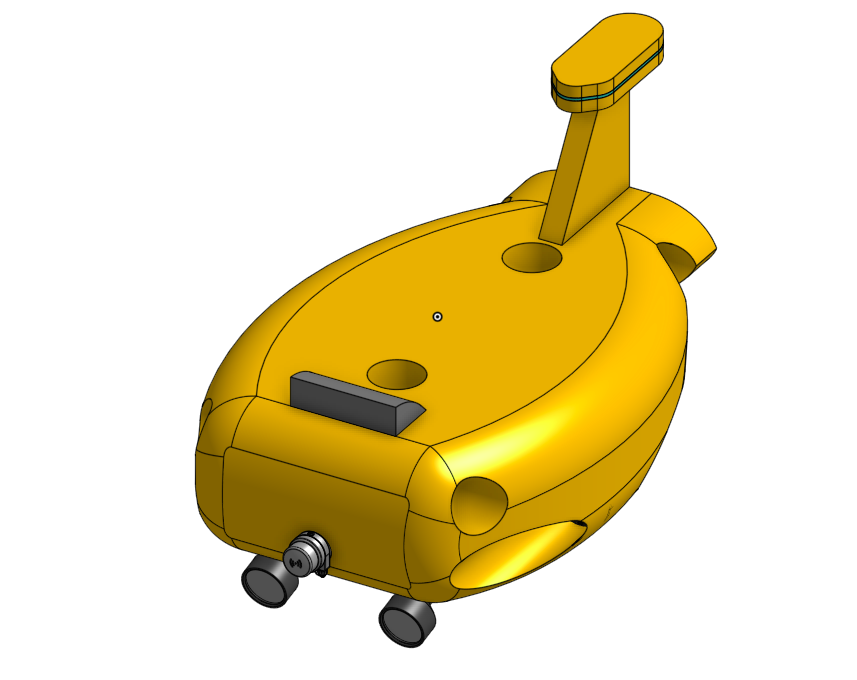
\includegraphics[trim = 0 20 0 50, clip, width=0.4\textwidth]{turbot-fish-01modi.png}
        %\caption{.}
    \end{figure}
%*----------- notes
    \note[item]{Notes can help you to remember important information. Turn on the notes option.}
\end{frame}
%-
%*----------- SLIDE -------------------------------------------------------------
\begin{frame}[t]{Objetivos}
    Objetivo Geral
    \newline
    Desenvolver um modelo de veículo submarino para a navegação em águas rasas.
    \newline

    Objetivos Específicos
    \begin{itemize}
        \item Realizar o estudo do estado da arte
        \item Realizar o desing da estrutura do submarino
        \item Realizae simuolações (CFD,ROS)
        \item Desenvolver o planejamento dos experimentos
        \item Desenvolver artigos científicos
    \end{itemize}
   

%*----------- notes
    \note[item]{Notes can help you to remember important information. Turn on the notes option.}
\end{frame}
%-
%*----------- SLIDE -------------------------------------------------------------
\begin{frame}[c]{Metodologia }
    %\transboxin[duration=1,direction=30]
        \begin{figure}
        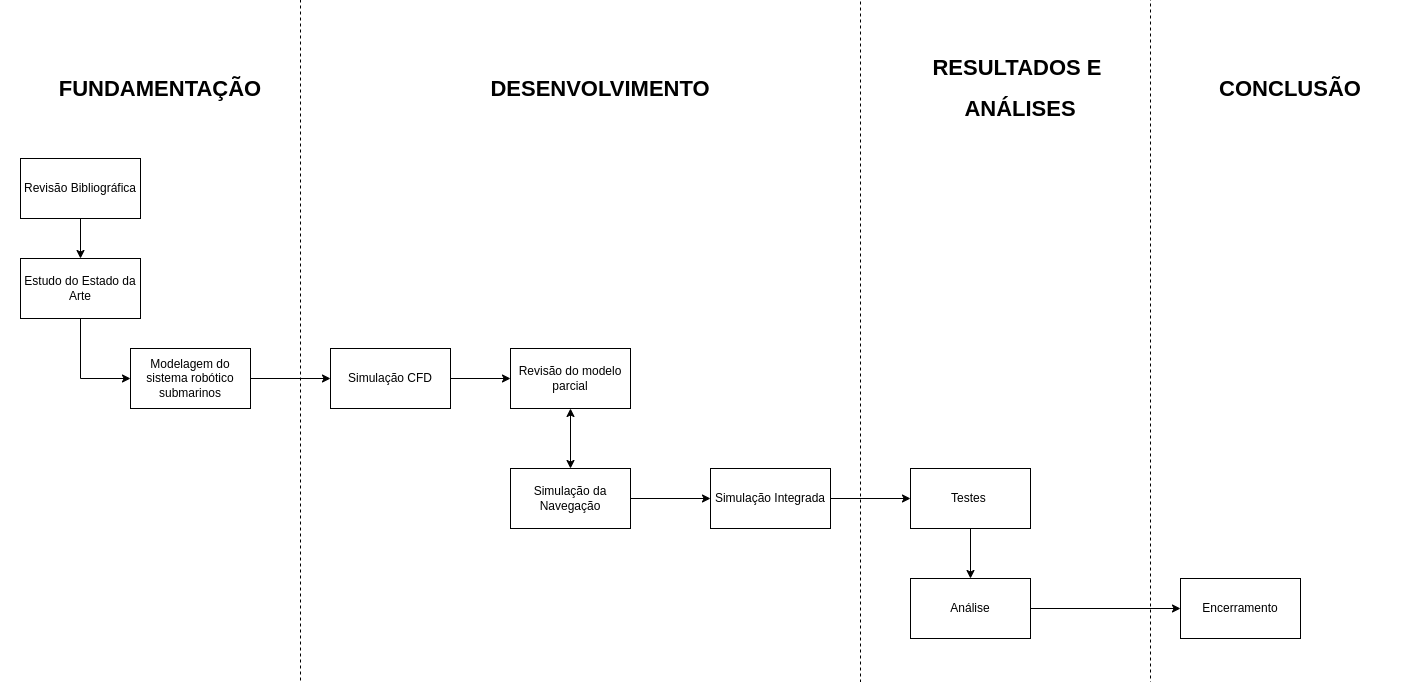
\includegraphics[width=.8\textwidth]{metodologiamodi.png}
    \end{figure}
%*----------- notes
    \note[item]{Notes can help you to remember important information. Turn on the notes option.}
\end{frame}
%-
%*----------- SLIDE -------------------------------------------------------------
\begin{frame}[t]{Método BiLi}
    \textbf{Ciclo Ingênuo} 
    \newline
        Foram pesquisados 10 ".bib" para chegar no resultado 
    \newline
        Palavras chaves: underwater vehicle,underwater robotics,cfd modeling,cfd simulation, OpenFOAM
    \newline
        Artigos encontrados: 633
    \newline
        String gereada: "underwater vehicle" OR "autonomous underwater" OR "operated vehicle" OR
        "remotely operated" OR "robotic vehicle" OR "underwater robot") AND ("computational fluid" OR "fluid dynamic") 
        AND ("control system" OR "fluid dynamics")
    \newline
    \textbf{Ciclo Otmizado}
    \newline
        Utilização do litserach para otimização da strin
    \newline
        Artigos encontrados: 733
    \newline
        Filtragem do RevTools: 357 artigos

%*----------- notes
    \note[item]{Notes can help you to remember important information. Turn on the notes option.}
\end{frame}
%-
%*----------- SLIDE -------------------------------------------------------------
\begin{frame}[t]{Ciclo Ingênuo X Ciclo Otmizado}
    \transboxout[duration=0.5]
    \framesubtitle{Taxa de crescimento anual de artigos científicos}
    
    \begin{columns}
        \column{.4\textwidth}
        \newline  
            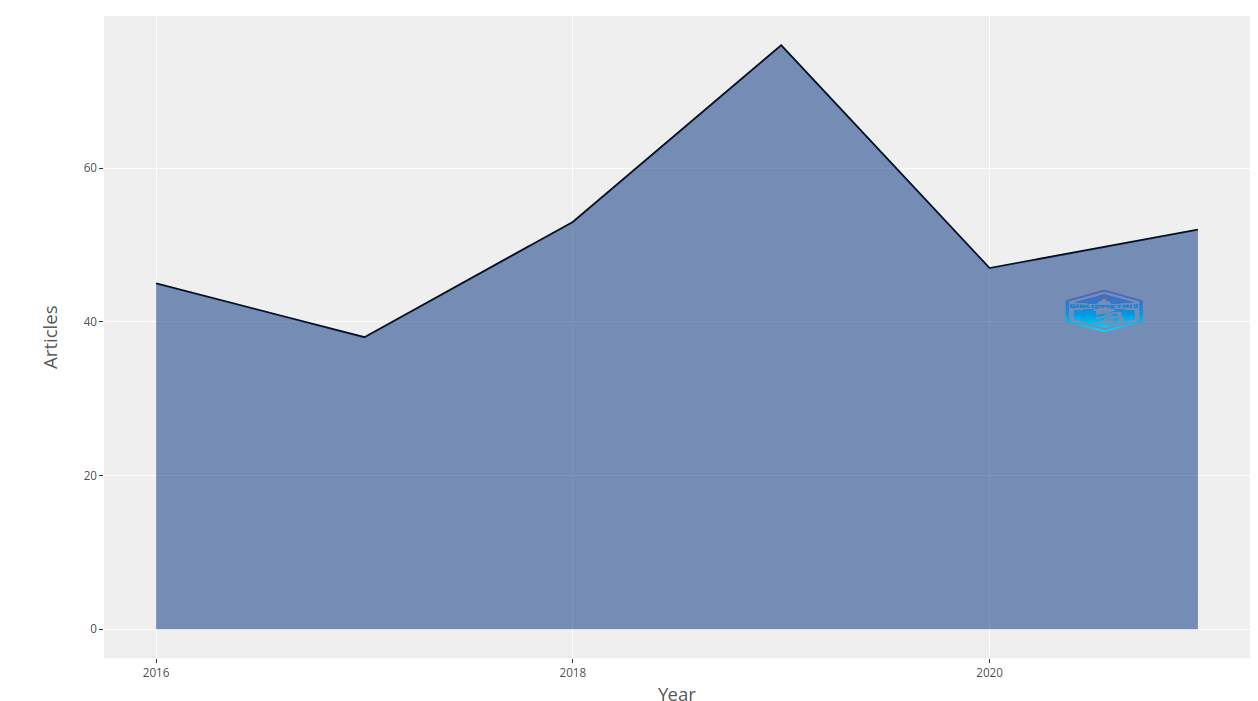
\includegraphics[height = 4cm, width=1.2\textwidth]{produçãoanual1.png}
        \column{.4\textwidth}
        \newline  
         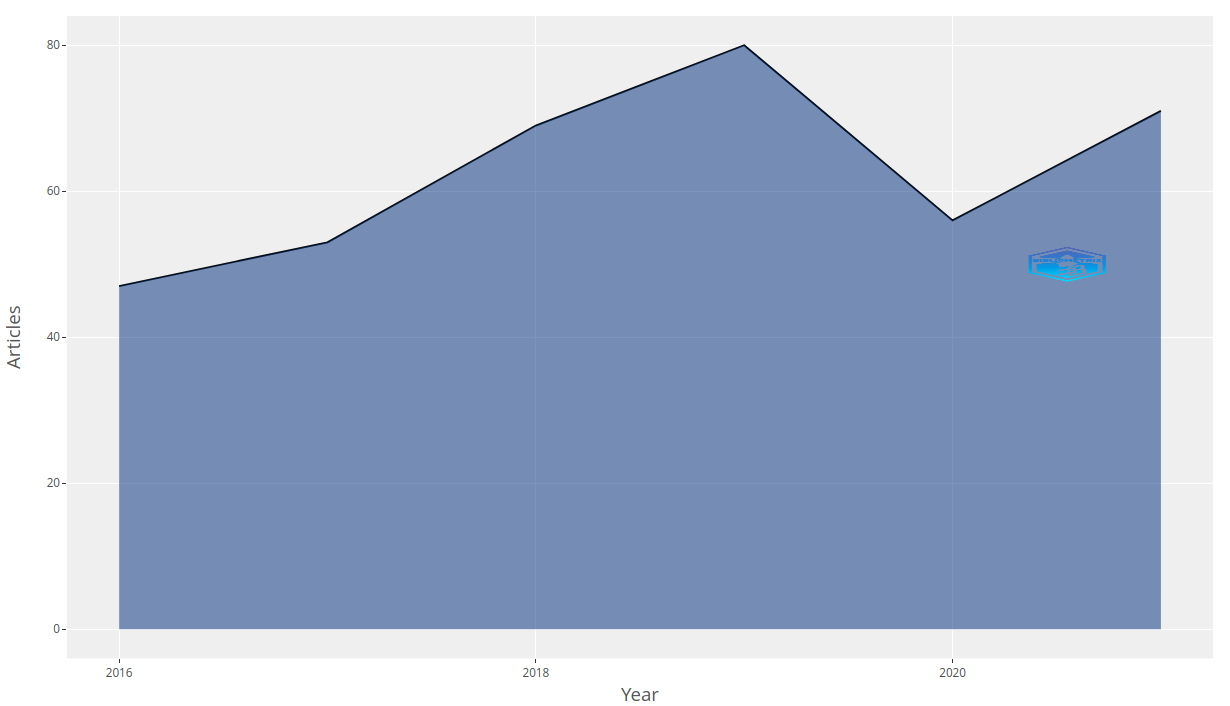
\includegraphics[height = 4cm, width=1.2\textwidth]{producaanual2.png}
    \end{columns}
    
    \begin{columns}
        \column{.4\textwidth}
        \newline  
        Taxa de crescimento: 2.93\%
        \column{.4\textwidth}
        \newline
         Taxa de crescimento: 8.6\%
    \end{columns}
 %*----------- notes
    \note[item]{Notes can help you to remember important information. Turn on the notes option.}
\end{frame}
%-
%*----------- SLIDE -------------------------------------------------------------
\begin{frame}[t]{Ciclo Ingênuo X Ciclo Otmizado}
    \transboxout[duration=0.5]
    \framesubtitle{Rede de co-citação}
    
    \begin{columns}
        \column{.4\textwidth}
        \newline  
            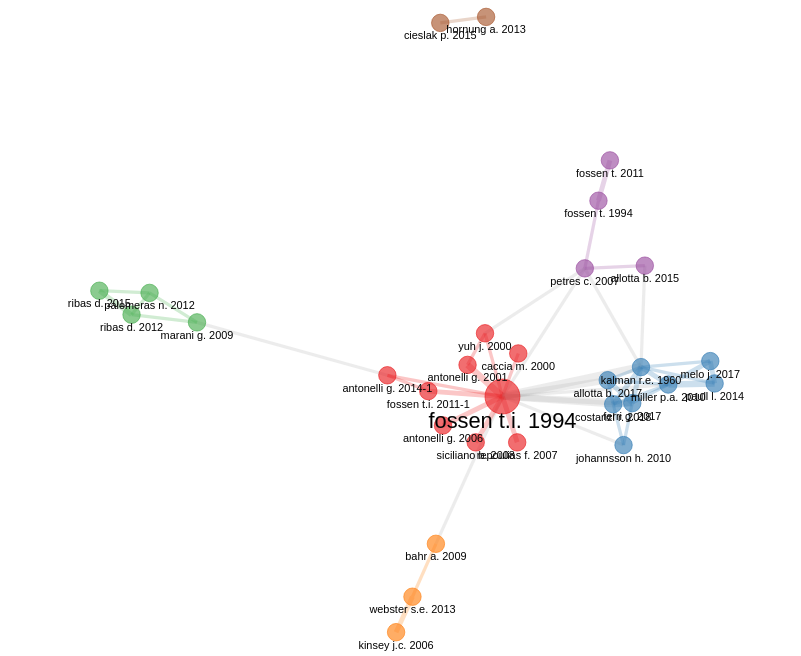
\includegraphics[height = 5cm, width=1.2\textwidth]{cocitação1.png}
        \column{.4\textwidth}
        \newline  
         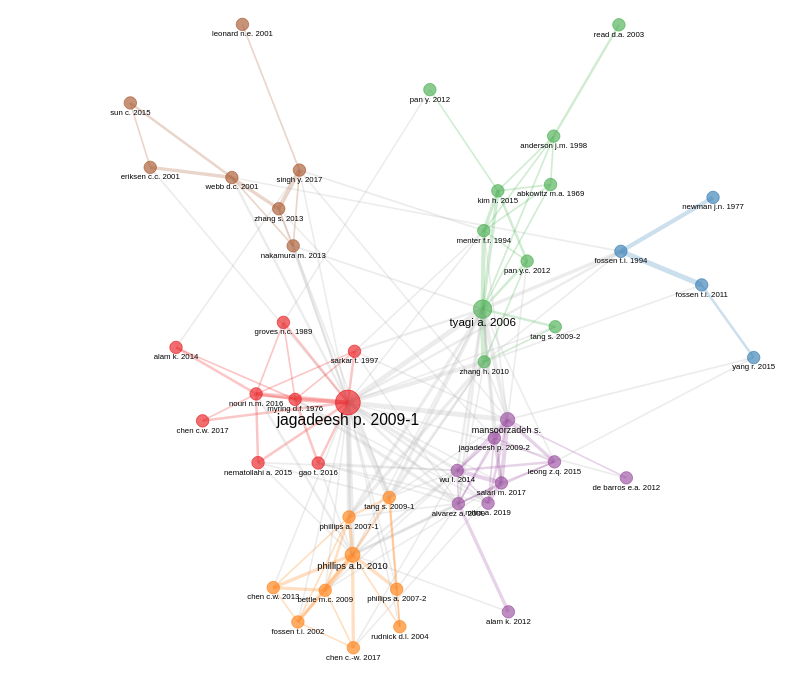
\includegraphics[height = 5cm, width=1.2\textwidth]{cocitação2.png}
    \end{columns}
    
 %*----------- notes
    \note[item]{Notes can help you to remember important information. Turn on the notes option.}
\end{frame}
%-
%*----------- SLIDE -------------------------------------------------------------
\begin{frame}[t]{Ciclo Ingênuo X Ciclo Otmizado}
    \transboxout[duration=0.5]
    \framesubtitle{Mapa de palavras}
    
    \begin{columns}
        \column{.4\textwidth}
        \newline  
            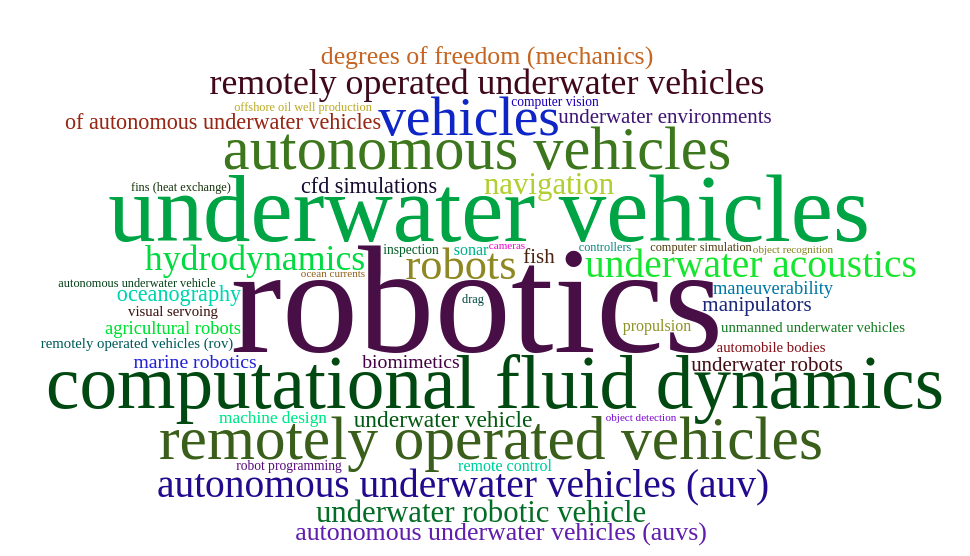
\includegraphics[height = 4cm, width=1.2\textwidth]{mapadepalavras1.png}
        \column{.4\textwidth}
        \newline  
         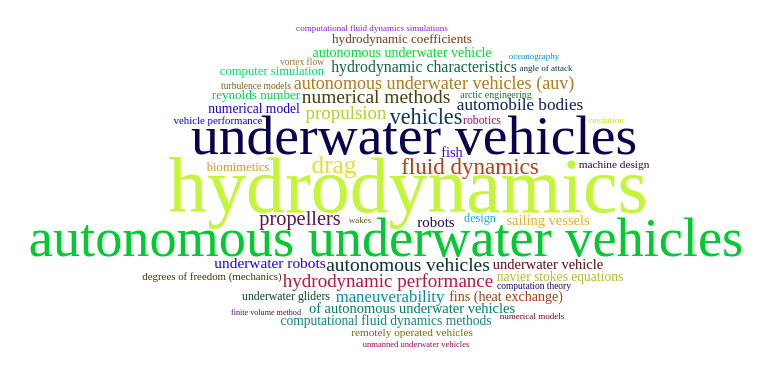
\includegraphics[height = 4cm, width=1.2\textwidth]{mapadepalavras2.png}
    \end{columns}
    
 %*----------- notes
    \note[item]{Notes can help you to remember important information. Turn on the notes option.}
\end{frame}
%-
%*----------- SLIDE -------------------------------------------------------------
\begin{frame}[c]{Cronograma}
    %\transboxin[duration=1,direction=30]
        \begin{figure}
        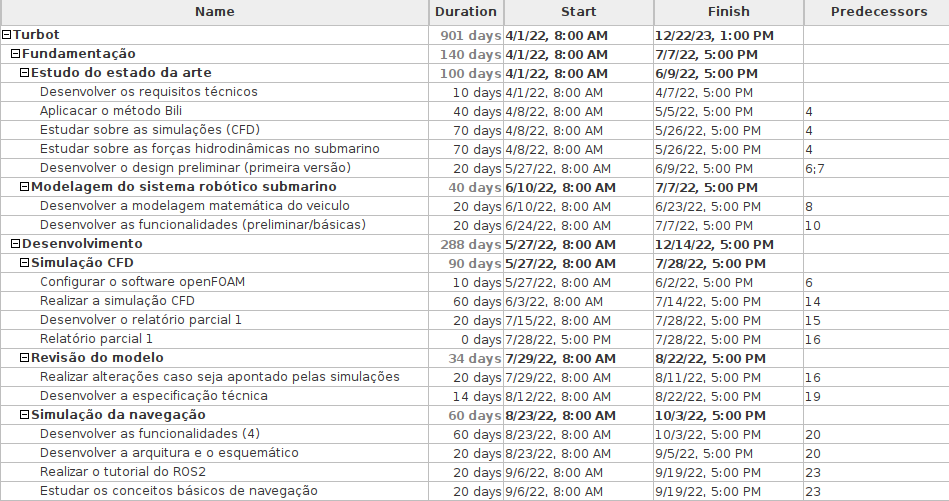
\includegraphics[width=.9\textwidth]{cronograma1.png}
    \end{figure}
%*----------- notes
    \note[item]{Notes can help you to remember important information. Turn on the notes option.}
\end{frame}
%-
%*----------- SLIDE -------------------------------------------------------------
\begin{frame}[c]{Cronograma}
    %\transboxin[duration=1,direction=30]
        \begin{figure}
        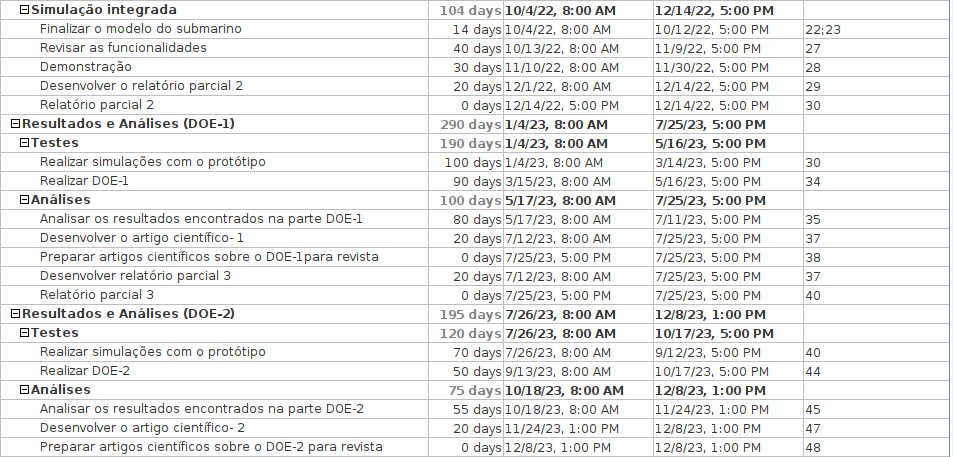
\includegraphics[width=.9\textwidth]{cronograma2.png}
    \end{figure}
%*----------- notes
    \note[item]{Notes can help you to remember important information. Turn on the notes option.}
\end{frame}
%-
%*----------- SLIDE -------------------------------------------------------------
\begin{frame}[c]{Cronograma}
    %\transboxin[duration=1,direction=30]
        \begin{figure}
        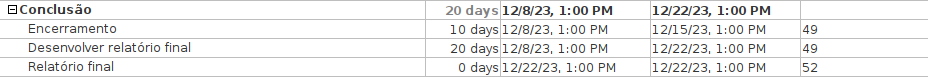
\includegraphics[width=1\textwidth]{cronograma3.png}
    \end{figure}
%*----------- notes
    \note[item]{Notes can help you to remember important information. Turn on the notes option.}
\end{frame}
%-